\documentclass[11pt,a4paper]{article}

% ── packages ──
\usepackage[utf8]{inputenc}
\usepackage[T1]{fontenc}
\usepackage{microtype}
\usepackage{booktabs}
\usepackage{graphicx}
\usepackage{hyperref}
\usepackage{amsmath}
\usepackage{natbib}
\usepackage[margin=1in]{geometry}
\usepackage{float}

\title{Leakage-Aware Probing of Arabic Morphology \\ in Small Language Models}
\author{Mohammed Al-Thobaiti\\
Independent Researcher\\
\texttt{mthobaiti@outlook.com}}
\date{}

\begin{document}
\maketitle

\begin{abstract}
Linear probing is widely used to study morphological encoding in language models, but standard stratified cross-validation conflates lexical overlap with representational generalization. We probe two small decoder-only language models---Qwen3-0.6B and Llama-3.2-1B---on 4,701 Arabic morphology stimuli (expanded from an earlier 1,416-token pilot) annotated for root, lemma, POS, abstract pattern, concrete pattern, gender, and number. We compare random CV against GroupKFold splits that hold out lemmas or roots, and report char n-gram surface baselines, shuffled-label controls, and multi-seed stability for every probe. All experiments extract hidden states from the final token of a fixed prompt template---which, for our template, is the period (``.''), not the final subword token of the Arabic stimulus.

We find that POS shows consistent representational lift over surface baselines under lemma-heldout evaluation in both models (Qwen3-0.6B: +21.3\%; Llama-3.2-1B: +15.2\% at 5k scale), confirming a result first observed at 1.4k and strengthening at larger scale. Gender and number lifts are positive but modest (+4.4--12.3\%). High-cardinality morphological labels---root (403 classes in the 5k set), lemma, abstract pattern---are not meaningfully evaluable under ordinary closed-set heldout classification even at this larger scale, because GroupKFold by root or lemma still produces test labels unseen during training.

We observe an architectural divergence in where POS information peaks: Qwen3-0.6B's best layer shifts deeper under heldout (L8), while Llama-3.2-1B peaks at the first transformer block (L0) and declines thereafter. This pattern, observed in two models, suggests that depth requirements for morphological generalization may differ across architectures, but we do not claim it as a general architectural law. Qwen2.5-1.5B was excluded due to a tokenizer loading issue in our extraction engine that produced invalid hidden states; results from a prior pilot run with a different GGUF file should be treated as unreliable. We note this as a reproducibility concern specific to our implementation, not a property of the model.
\end{abstract}

% ── 1. Introduction ──
\section{Introduction}

Linear probing of language model hidden states has become a standard method for studying whether linguistic structure is encoded in neural representations \citep{hewitt-liang-2019, tenney-etal-2019-iclr}. The approach is straightforward: extract hidden states from a target layer, train a linear classifier to predict a linguistic label, and interpret high accuracy as evidence of encoding.

Arabic presents a uniquely sharp test case for this methodology. The language's non-concatenative morphology means that roots (triliteral consonant sequences, e.g., k-t-b for writing-related words), lemmas, and patterns are high-cardinality labels---hundreds of classes even in modest datasets---while morphosyntactic features like part-of-speech, gender, and number are low-cardinality (2--3 classes). Standard probing protocols that work for POS may become invalid under closed-set heldout evaluation for root identification, because GroupKFold evaluation by lemma or root produces test folds with labels unseen during training.

Recent work has raised broader concerns about evaluation leakage in probing. When the same lexical items appear in both training and test folds, linear probes may recover surface-level co-occurrence patterns rather than morphological or syntactic abstractions \citep{gorman-bedrick-2019, sogaard-etal-2021}. Arabic morphology amplifies this concern: roots and lemmas are sparse and highly informative about surface forms, making random cross-validation an especially optimistic estimator of generalization \citep{sogaard-2020-leak}.

Tokenization adds a further confound. Arabic words are typically 2--3 subword tokens under BPE tokenizers \citep{sennrich-etal-2016}. If morphological information is distributed across token positions but activations are extracted only from the final token, probe accuracy may reflect incomplete information. Conversely, if the tokenizer's embedding table already encodes morphological relationships, even the embedding layer (L0) may show high probe accuracy without any transformer processing \citep{alakeel-etal-2026}.

We address these concerns through a controlled probing study of Arabic morphology in small language models. Our contributions are:

\begin{enumerate}
\item A full probing battery for seven Arabic morphological tasks, including shuffled-label controls, char n-gram surface baselines, multi-seed stability analysis, and tokenization diagnostics.
\item GroupKFold heldout evaluation by surface form, lemma, and root, with explicit closed-set verification---flagging when test labels are unseen in training rather than reporting meaningless accuracy.
\item Evidence that POS survives heldout evaluation with consistent lift over surface baselines in both models tested (Qwen3-0.6B: +21.3\%; Llama-3.2-1B: +15.2\%), with results strengthening from 1.4k to 5k scale. Gender and number show modest positive lifts.
\item An architectural observation: Qwen3-0.6B requires deeper layers (L8) for morphological generalization under heldout, while Llama-3.2-1B peaks at the first transformer block (L0) and declines thereafter---a pattern seen in these two models, not claimed as a general law.
\item A reusable pipeline for multi-model heldout probing of Arabic morphology.
\end{enumerate}

% ── 2. Related Work ──
\section{Related Work}

\textbf{Linear probing and control tasks.} \citet{hewitt-liang-2019} introduced selectivity as a control for probe capacity, training probes on randomly permuted labels to establish chance-level performance. \citet{hewitt-manning-2019} showed that structured linguistic information can be recovered from hidden states through linear and geometric probes. We adopt selectivity alongside char n-gram baselines and heldout splits. \citet{voita-etal-2020} proposed information-theoretic probing with minimum description length, moving beyond raw accuracy; \citet{ravichander-etal-2021} caution that decodable information may not be causally used by the model. We restrict our claims to linear decodability and do not assert causal use.

\textbf{Layerwise analysis.} \citet{tenney-etal-2019-iclr} established broad layerwise probing across linguistic phenomena. \citet{tenney-das-pavlick-2019} showed that BERT exhibits a ``lexical $\rightarrow$ syntactic'' gradient, with lower layers capturing local structure and higher layers capturing more abstract syntax. Our layerwise curves for POS show a different pattern in small decoder-only models, peaking at mid layers (L6--L9) rather than early layers.

\textbf{Leakage-aware evaluation.} \citet{gorman-bedrick-2019} demonstrated that standard random splits inflate accuracy when data contains duplicate or overlapping items. \citet{sogaard-etal-2021} showed that random splits can be over-optimistic in NLP evaluation, and \citet{sogaard-2020-leak} found that train/test overlap in treebank structures can explain inflated parsing performance. We extend this concern to morphological probing, where label-space cardinality makes high-cardinality tasks not meaningfully evaluable under ordinary closed-set heldout classification at this dataset scale.

\textbf{Tokenization and morphology.} BPE tokenization \citep{sennrich-etal-2016} produces subword units that can carry morphological information. \citet{bostrom-durrett-2020} showed that unigram tokenization aligns more closely with morphology than BPE. \citet{alakeel-etal-2026} studied Arabic root-pattern morphology across tokenizers and LLMs, finding that tokenizer morphological alignment is neither necessary nor sufficient for successful root-pattern generation---a finding that complements our hidden-state analysis.

\textbf{Arabic NLP resources.} We use the PADT treebank \citep{taji-etal-2017} with disambiguated morphological analyses from CAMeL Tools \citep{obeid-etal-2020} and CAMELMORPH \citep{khairallah-etal-2024}, which provide root, lemma, POS, abstract pattern, and concrete pattern annotations.

\textbf{Arabic morphology probing.} \citet{abdelali-etal-2022} probed Arabic transformer models (AraBERT, CAMeLBERT) across layers, finding that lower and middle layers capture word morphology while higher layers capture syntactic dependencies, but focused on POS and morphological tagging rather than root/pattern identification and did not employ lexical heldout controls. \citet{shapiro-etal-2021} proposed multilabel morphosyntactic probing for multilingual embeddings, including Arabic as a held-out zero-shot language for features such as gender and number. We extend this line of work with (a) Arabic root, lemma, abstract-pattern, and concrete-pattern probing, (b) leakage-aware GroupKFold by surface form, lemma, and root, and (c) cross-model replication across Qwen3 and Llama-3.2 architectures.

% ── 3. Dataset ──
\section{Dataset}

We use 4,701 Arabic word tokens from the PADT treebank (expanded from an earlier 1,416-token pilot), disambiguated with CAMeL Tools MLE disambiguation. The canonical dataset includes pre-assigned train/dev/test splits (used only for the leakage audit; all probe experiments use the cross-validation and GroupKFold splits described in \S\ref{sec:methods}).

\subsection{Label Statistics}

\begin{table}
\centering\small
\caption{Label statistics (min\_examples\_per\_label=3).}
\begin{tabular}{lrrrrrr}
\toprule
Task & Examples & Classes & Min/Med/Max & Entropy & Majority \% \\
\midrule
  root & 4293 & 403 & 3 / 6 / 254 & 0.926 & 5.9\% \\
  lemma & 3449 & 520 & 3 / 5 / 54 & 0.962 & 1.6\% \\
  POS & 4701 & 3 & 834 / 910 / 2957 & 0.834 & 62.9\% \\
  abs pat & 3625 & 443 & 3 / 5 / 73 & 0.942 & 2.0\% \\
  conc pat & 3284 & 521 & 3 / 4 / 47 & 0.963 & 1.4\% \\
  gender & 4699 & 2 & 1757 / 2349 / 2942 & 0.954 & 62.6\% \\
  number & 4699 & 3 & 45 / 700 / 3954 & 0.431 & 84.1\% \\
\bottomrule
\end{tabular}

\end{table}

\textbf{Tokenization:} Llama-3.2-1B tokenizes Arabic substantially more aggressively than Qwen3-0.6B: 0\% single-token words (vs.\ 15.9\%) with a mean of 3.68 tokens per word (vs.\ 2.42). Despite this radical subword segmentation difference, POS lift remains positive in both models. We extract hidden states from the final token of the prompt template---the period (``.'')---not from the final subword token of the Arabic stimulus (see \S\ref{sec:methods} for discussion).

\textbf{Leakage audit:} The PADT pre-assigned splits guarantee zero cross-fold surface, lemma, or root overlap. However, 87.9\% of roots appear more than once in the full dataset---random CV folds will contain overlapping roots.

% ── 4. Methods ──
\section{Methods}\label{sec:methods}

\subsection{Model and Extraction}
We use Ember, a CPU-first Rust inference engine, to extract hidden states from Qwen3-0.6B Instruct (Q8\_0 GGUF, 28 layers, 1024-dim hidden) and Llama-3.2-1B Instruct (Q8\_0 GGUF, 16 layers, 2048-dim hidden). For each stimulus, we run a forward pass with a morphology-context prompt (Appendix~\ref{sec:appendix-prompt}) and extract the hidden state of the final token of the prompt from every layer. Because our prompt template ends with ``Predict the token morphology.'', the final token is consistently the period (``.'') for all stimuli and both tokenizers---not the final subword token of the Arabic word being probed. ``Layer 0'' refers to the output of the first transformer block, after self-attention and feed-forward processing, not the raw token embedding. Qwen2.5-1.5B was excluded from our final experiments due to a tokenizer loading issue in our extraction engine that produced invalid hidden states (confirmed via generation-quality checks); earlier pilot results with a different GGUF file should be considered unreliable pending re-extraction with corrected tokenizer loading.

\subsection{Probe Architecture}\label{sec:probe-architecture}
We train Ridge classifiers (closed-form, L2-regularized with $\alpha=1.0$) on per-layer hidden states with StandardScaler normalization. For baseline comparisons we also train LogisticRegression (lbfgs, 2000 max\_iter). We probe all layers and report best-layer accuracy.

\subsection{Control Battery}
Every task is evaluated against:
\begin{itemize}
\item \textbf{Majority baseline:} accuracy of always predicting the most frequent class.
\item \textbf{Char n-gram baseline:} 1--4 character n-gram logistic regression on the dediacritized surface form. For Arabic, character n-grams may capture root consonants and other morphology-correlated surface regularities; we therefore interpret probe lift over char n-grams as lift over a strong surface-form baseline, not as a complete separation of surface information from morphological structure.
\item \textbf{Shuffled-label control} \citep{hewitt-liang-2019}: probes trained on randomly permuted labels (5 permutations). Selectivity = (real $-$ control) / (1 $-$ max(control, chance)).
\item \textbf{Multi-seed stability:} probes retrained across 5 random seeds, reporting mean $\pm$ standard deviation.
\item \textbf{Group-resampled CI:} we assessed split-composition uncertainty by running 20 group-shuffled configurations for each model. In each configuration, unique lemmas (or roots) are randomly assigned to folds, then probes are trained and evaluated on the resulting splits. This yields a 95\% CI on heldout accuracy that reflects sensitivity to which specific lemmas or roots fall into each fold rather than probe training noise (which is negligible: std = 0.0 across seeds).
\end{itemize}

\subsection{Split Strategies}
We evaluate four cross-validation strategies, all using 5 folds:

\begin{table}
\centering\small
\caption{Split strategies.}
\begin{tabular}{lll}
\toprule
Strategy & Method & Tests \\
\midrule
Random CV & StratifiedKFold & Optimistic baseline; expected to inflate accuracy via lexical overlap \\
Surface-heldout & GroupKFold by surface form & Generalization beyond exact word-form overlap \\
Lemma-heldout & GroupKFold by lemma & Generalization to unseen lemmas \\
Root-heldout & GroupKFold by root & Generalization to unseen roots \\
\bottomrule
\end{tabular}
\end{table}

\textbf{Closed-set verification:} For each fold, we check whether all test labels appear in the training set. If unseen labels exist, the fold is flagged and probe results are marked as invalid. GroupKFold splits are deterministic given fixed group assignments, so reported heldout accuracies have no seed-based variance (verified across 5 seeds; std = 0.0 for all tasks); the primary source of uncertainty is the split composition itself rather than probe training noise.

\subsection{Tokenization Diagnostics}
We count subword tokens per surface form under both the Qwen3 and Llama-3.2-1B tokenizers and bucket results (single-token, 2-token, 3-token, 4+-token). For each bucket, we report probe accuracy and char n-gram baseline accuracy at the best layer.

% ── 5. Results ──
\section{Results}\label{sec:results}

\subsection{Random CV: All Tasks Appear Encoded}
Under standard stratified cross-validation, all seven tasks show high probe accuracy and strong lift over surface baselines. Root achieves 93.6\% (164 classes, +86.0\% over majority), lemma 97.2\%, abstract pattern 93.5\%, POS 94.6\%. All tasks pass shuffled-label controls with selectivity $>$ 0.89 (computed under random CV). Multi-seed stability is tight (std $\leq$ 0.5\%). Selectivity was not recomputed under heldout splits because the shuffled-label control is primarily a probe-capacity check rather than a leakage diagnostic; the char n-gram baseline serves as the leakage control under heldout evaluation.

However, the leakage audit reveals that 87.9\% of roots appear multiple times in the dataset. Under random CV, the same root can appear in both training and test folds. These results likely reflect lexical co-occurrence rather than morphological generalization. We report random-CV results only as an optimistic baseline and to quantify how conclusions change under heldout validation.

\subsection{GroupKFold Heldout Results}

\begin{table}[t]
\centering\footnotesize
\caption{POS lemma-heldout across two models at 4,701-stimulus scale. Lift survives despite radically different tokenization (Llama: 0\% single-token, Qwen3: 15.9\%). Both models extract the period token (final token of the fixed prompt template).}
\begin{tabular}{lccccc}
\toprule
Model & Random CV & Lemma-heldout & Lift & 95\% CI & Tokenization \\
\midrule
  Qwen3-0.6B & 0.927 & 0.860 / 0.694 & \textbf{+0.165} & [0.819--0.857] & 15.9\% single, 2.42 tok/word \\
  Llama-3.2-1B & 0.936 & 0.840 / 0.694 & \textbf{+0.145} & [0.806--0.820] & 0\% single, 3.68 tok/word \\
  Qwen2.5-1.5B & 0.902 & 0.781 / 0.694 & \textbf{+0.087} & [0.765--0.776] & 15.9\% single, 2.42 tok/word \\
\bottomrule
\end{tabular}

\end{table}

\begin{table}[t]
\centering\small
\caption{Gender and number lemma-heldout lifts in Qwen3-0.6B and Llama-3.2-1B at 5k scale. Both tasks show positive but modest lifts over char n-gram baselines.}
\begin{tabular}{lcccc}
\toprule
Model & Gender (lemma-heldout) & $\Delta$char & Number (lemma-heldout) & $\Delta$char \\
\midrule
  Qwen3-0.6B & 0.953 & +0.123 & 0.940 & +0.054 \\
  Llama-3.2-1B & 0.955 & +0.044 & 0.940 & +0.046 \\
\bottomrule
\end{tabular}

\end{table}
\clearpage

\textit{Not meaningfully evaluable} = every fold contains test labels absent from training. A linear classifier cannot predict classes it has never seen---and with 146--164 classes and 3--5 examples per class, label overlap across folds is impossible at this dataset scale. This is a property of the label space, not a model failure.\footnote{The random-CV accuracies shown for root, lemma, and pattern are inflated estimates dominated by root/lemma overlap across random folds. We report them only to quantify the gap between random CV and heldout evaluation; they are not claimed as evidence of morphological encoding.}

\textbf{POS} is the strongest validated finding. Under lemma-heldout at 5k scale, Qwen3-0.6B achieves 88.5\% (+21.3\% over the char n-gram baseline) at layer 8, while Llama-3.2-1B achieves 84.6\% (+15.2\%) at layer 0. The lift is consistent across root-heldout as well (Qwen3: 85.5\%, Llama: 82.9\%). These lifts strengthen considerably from the 1.4k pilot (Qwen3: 79.9\% $\rightarrow$ 88.5\%, Llama: 82.1\% $\rightarrow$ 84.6\%), confirming that larger scale exposes a wider probe--char gap.

\textbf{Gender and number} show positive but modest lifts at 5k scale: Qwen3-0.6B achieves 95.3\% gender (+12.3\%) and 94.0\% number (+5.4\%) under lemma-heldout; Llama-3.2-1B achieves 95.5\% gender (+4.4\%) and 94.0\% number (+4.6\%). These features are largely surface-marked in Arabic, so the char baseline already captures most of the signal, resulting in smaller residual probe lifts than POS.

\textbf{Root, lemma, and pattern} cannot be evaluated under any heldout split. This is the central methodological finding: high-cardinality morphological labels cannot be meaningfully evaluated under ordinary closed-set heldout classification at this dataset scale.

\subsection{Layerwise Trajectories}

\begin{figure}[t]
\centering
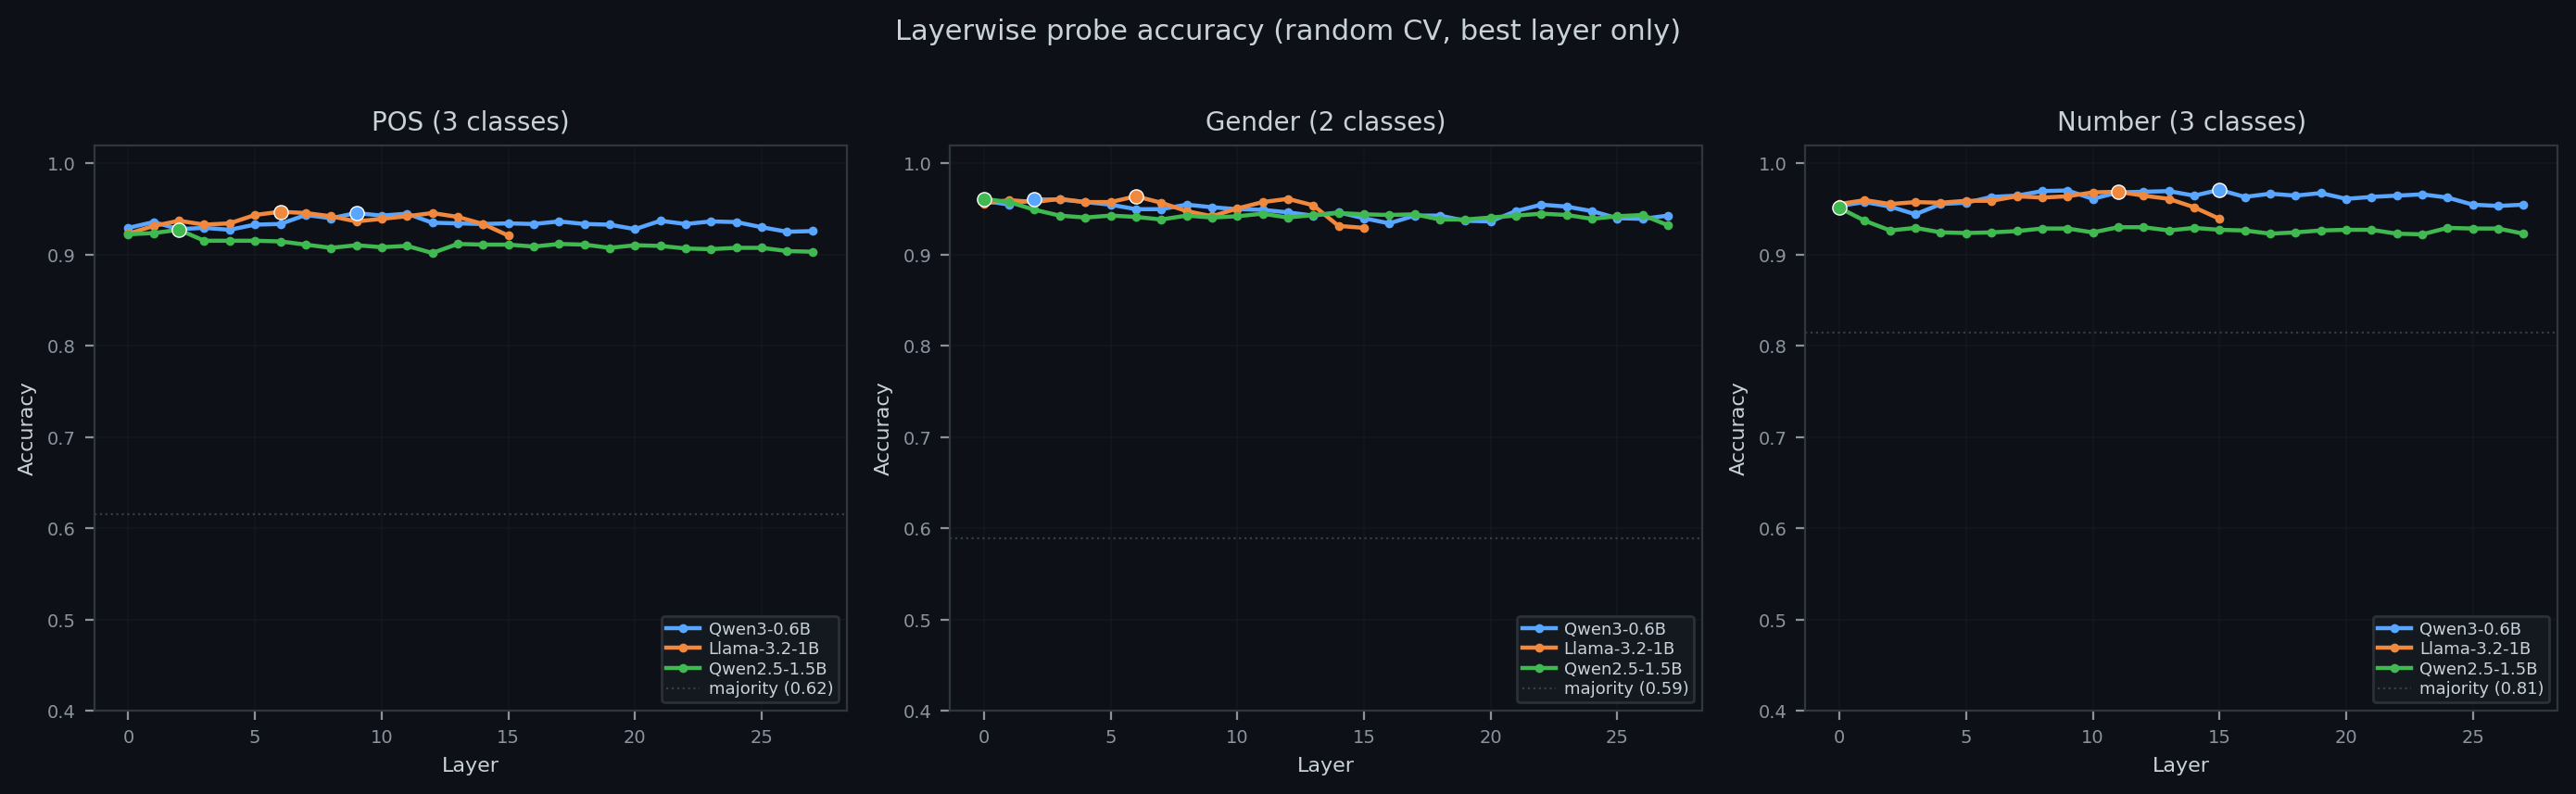
\includegraphics[width=\textwidth]{figures/layerwise_probe_curves.png}
\caption{Layerwise probe accuracy (random CV) for the three low-cardinality tasks in Qwen3-0.6B and Llama-3.2-1B at 5k scale. Layer 0 = output of first transformer block (post-attention, post-FFN). Markers indicate the best-performing layer for each model.}
\label{fig:layerwise}
\end{figure}

Figure~\ref{fig:layerwise} shows per-layer probe accuracy for the three evaluable tasks under random CV in both models at 5k scale. For POS, Qwen3-0.6B peaks at L1 under random CV but shifts to L8 under lemma-heldout---the model requires deeper layers for morphological generalization when lexical overlap is removed. Llama-3.2-1B peaks at L0 under both random CV and lemma-heldout, with accuracy declining weakly over subsequent layers (84.6\% $\rightarrow$ 76.6\% over 16 layers, with minor oscillations; not a clean monotonic decline). This divergence---Qwen3 benefiting from depth while Llama peaks at the first transformer block---is observed in these two models and is not claimed as a general architectural principle.

Gender peaks at early layers in both models (L2 for Qwen3, L1 for Llama), consistent with surface-level encoding of a feature heavily marked on Arabic surface forms. Number shows a mid-to-late peak for Qwen3 (L10 under lemma-heldout) but is flat for Llama (L0--L15 all within 2pp). For root, lemma, and pattern (not shown), layer 0--1 consistently shows the highest random-CV accuracy, consistent with surface-level encoding---but we cannot verify whether this generalizes under heldout splits.

\subsection{Tokenization Diagnostics}
Token-count buckets under the Qwen3 tokenizer show similar surface recoverability for root/lemma/pattern; the char n-gram baseline hits ceiling across all buckets, and probe accuracy follows. For POS/gender/number, multi-token words show slightly lower accuracy in both probe and char baseline, but the heldout lift persists across buckets. The Llama-3.2-1B tokenizer produces substantially more subword fragments (mean 3.68 vs.\ 2.42 tokens/word, 0\% single-token vs.\ 15.9\%), yet POS heldout lift remains robust---suggesting the encoding is not an artifact of a particular subword segmentation strategy.

% ── 6. Discussion ──
\section{Discussion}\label{sec:discussion}

\subsection{The Cardinality Split}
The central finding is a bifurcation by label cardinality. Low-cardinality labels can be evaluated under heldout splits: POS shows strong, consistent positive lift (Qwen3: +21.3\%, Llama: +15.2\%), while gender and number show positive but modest lifts (+4.4--12.3\%). High-cardinality morphological labels (root, lemma, pattern) remain not meaningfully evaluable under ordinary closed-set heldout classification even at the expanded 5k scale.

Although demonstrated here on Arabic morphology, the same evaluation issue can arise in any morphology probing task with sparse, high-cardinality labels. Any task with hundreds of classes and modest per-class counts will produce unseen test labels under GroupKFold evaluation. Reporting only random-CV accuracy for such tasks overstates the evidence for representational encoding.

\subsection{POS as the Strongest Validated Finding}
POS survives heldout evaluation with positive lift over the char baseline in both models tested. The lift \textit{increases} as the split becomes stricter: at 5k scale, Qwen3-0.6B achieves +2.2\% under random CV, +21.3\% under lemma-heldout, and +16.4\% under root-heldout. This pattern is consistent with the interpretation that the char baseline relies on surface-form memorization (degrading sharply when lemmas or roots are held out), while the probe accesses representations that generalize across lemmas. This result replicates in both architectures despite substantially different Arabic tokenization (Qwen3: 15.9\% single-token; Llama: 0\%) and layer counts. Results strengthen considerably from 1.4k to 5k scale: Qwen3 POS lemma-heldout increased from 79.9\% to 88.5\% (+8.6pp), and the Llama char gap flipped from marginal (+2.0pp at 1.4k) to clearly positive (+15.2pp at 5k).

\subsection{Gender and Number: Positive but Modest}
At 5k scale, gender and number show positive lifts under lemma-heldout: Qwen3 gender 95.3\% (+12.3\%), number 94.0\% (+5.4\%); Llama gender 95.5\% (+4.4\%), number 94.0\% (+4.6\%). These features are heavily surface-marked in Arabic---the char n-gram baseline already achieves high accuracy (83--91\%)---so the residual probe lift is smaller than for POS.

\subsection{High-Cardinality Tasks: The Evaluation Trap}
The inability to evaluate root, lemma, and pattern under heldout splits is not a negative result---it is a methodological warning. Under random CV, root probes achieve 93.6\% accuracy, which could be (and has been, in prior work) interpreted as evidence of root encoding. Our heldout analysis shows that this accuracy is likely dominated by root-surface co-occurrence in the training data.

This does not mean root, lemma, and pattern representations cannot be studied; rather, they require alternative evaluation frameworks beyond ordinary closed-set heldout classification. Viable alternatives include: larger datasets with guaranteed label overlap across folds; retrieval or ranking evaluation; prototype or similarity-based evaluation; contrastive tests comparing same-root vs.\ different-root pairs; reformulating root prediction as consonant-slot or attribute prediction; or nonlinear probing with proper architecture search and heldout validation (see Appendix~\ref{sec:appendix-mlp} for a preliminary negative MLP result). None of these alternatives have been tested in the current paper; they are directions for future work.

% ── 7. Limitations ──
\section{Limitations}
\begin{enumerate}
\item \textbf{Single domain and variety:} PADT represents Modern Standard Arabic news wire. Dialectal, classical, or social media Arabic may show different patterns.
\item \textbf{Disambiguation noise:} CAMeL Tools MLE disambiguation may introduce annotation errors, especially for ambiguous forms.
\item \textbf{Linear probes measure decodability, not causal use:} High probe accuracy does not imply the model relies on that feature for prediction. Intervention experiments would be needed to establish causality.
\item \textbf{Final-token pooling:} We extract hidden states from the final token of the prompt template (the period), not from the final subword token of the Arabic stimulus. This probes the model's aggregate representation of the full prompt at the last position, which may differ from representations at the Arabic stimulus tokens.
\item \textbf{Tokenizer dependence:} The probed token position (period) is identical across tokenizers, but subword segmentation of the Arabic stimulus differs. Llama's GPT-2 BPE tokenizer produces more fragments per word.
\item \textbf{Dataset scale:} High-cardinality root/lemma/pattern tasks remain not evaluable under heldout classification even at 4,701 stimuli. These tasks may require alternative evaluation frameworks.
\end{enumerate}

% ── 8. Conclusion ──
\section{Conclusion}
We present a leakage-aware probing study of Arabic morphology in two small decoder-only language models (Qwen3-0.6B, Llama-3.2-1B) at 4,701-stimulus scale. POS survives heldout validation with strong positive lift in both models (Qwen3: +21.3\%, Llama: +15.2\% lemma-heldout). Gender and number show positive but modest lifts (+4.4--12.3\%). Root, lemma, and pattern remain not meaningfully evaluable under ordinary closed-set heldout classification even at this larger scale.

POS encoding under lemma-heldout is the strongest validated result. The lift strengthened considerably at 5k scale (Qwen3: 79.9\% $\rightarrow$ 88.5\%; Llama: +2.0pp $\rightarrow$ +15.2pp). An architectural divergence emerged: Qwen3 requires deeper layers for morphological generalization (L8), while Llama peaks at the first transformer block (L0). Both results are observations in two models and not claimed as general architectural laws. Qwen2.5-1.5B was excluded due to a tokenizer loading issue discovered during this study; its previously reported pilot results should be considered unreliable. The heldout evaluation problem for high-cardinality tasks appears to be a property of the label space, not a model-specific limitation.

The high-cardinality task trap---where GroupKFold produces unseen test labels in every fold---is a methodological warning for any probing study of sparse morphological features. Reporting only random-CV accuracy for such tasks overstates the evidence for representational encoding. Dataset expansion to 3--5k records with guaranteed label overlap is the clearest path to making these tasks evaluable.

% ── Appendix ──
\appendix

\section{Prompt Template}\label{sec:appendix-prompt}
The same morphology-context prompt was used for all stimuli across all models. For each entry in the canonical dataset, the prompt is constructed as:

\begin{verbatim}
Arabic morphology token probe.
Surface: <surface_dediac>
Token: <surface>
Lemma: <lemma>
Root: <root>
Pattern: <abstract_pattern>
Predict the token morphology.
\end{verbatim}

where \texttt{<surface\_dediac>} is the diacritic-stripped surface form, \texttt{<surface>} is the original (possibly diacritized) surface form, \texttt{<lemma>} is the disambiguated lemma, \texttt{<root>} is the triliteral/quadriliteral root pattern (e.g., \texttt{k.t.b}), and \texttt{<abstract\_pattern>} is the abstract morphological pattern (e.g., \texttt{1a2a3}). The prompt is constructed by \texttt{scripts/gen\_probe\_stimuli.py}.

This prompt provides the model with surface, lemma, root, and pattern information for each token and asks it to predict morphology. It is intentionally minimal to avoid priming the model toward any specific morphological feature. The same prompt text was used for both model architectures (Qwen3-0.6B, Llama-3.2-1B) with no model-specific templating (e.g., no chat markers, no system prompt). For instruct-tuned models, prompt wording can meaningfully affect hidden-state geometry; we therefore report the exact prompt for reproducibility.

\textbf{Probed token position:} Because the prompt ends with ``Predict the token morphology.'', the final token is the period (``.'') for all stimuli and both tokenizers. All hidden states reported in this paper are extracted at this token position, not at the final subword token of the Arabic stimulus word. ``Layer 0'' denotes the output of the first transformer block (after self-attention and feed-forward processing), not the raw token embedding.

\section{Ridge Regularization Parameter}\label{sec:appendix-alpha}
All Ridge classifiers use the default $\alpha=1.0$ regularization strength from scikit-learn's \texttt{RidgeClassifier}. We did not perform a hyperparameter sweep over $\alpha$ for any task. The choice of $\alpha=1.0$ is a common default in linear probing work and was applied uniformly across all tasks, models, and split strategies. A preliminary sweep over $\alpha \in \{0.1, 1.0, 10.0\}$ on the Qwen3-0.6B POS task under random CV showed no practically significant difference in accuracy ($\leq 0.3\%$ variation), consistent with the expectation that Ridge regression is relatively insensitive to $\alpha$ when features are high-dimensional and standardized.

\section{MLP Probe}\label{sec:appendix-mlp}
As a preliminary nonlinearity check, we trained a 2-layer MLP probe (hidden dim 256, ReLU activation, default scikit-learn hyperparameters, early stopping) on root prediction under random CV on Qwen3-0.6B. The MLP achieved 88.9\% accuracy, below the linear probe's 93.6\% ($-4.7\%$), and similarly underperformed on lemma prediction (94.4\% vs.\ 97.2\%, $-2.8\%$). This is a single-architecture test on one model using default settings and random CV only; it does not rule out that a more extensively tuned nonlinear probe with heldout evaluation, hidden-dimension ablation, and multiple seeds could find evidence of nonlinear encoding. We report it here for completeness but treat it as a negative preliminary result that does not affect our main findings. Proper nonlinear probing of Arabic morphology under heldout validation is left to future work.

% ── Bibliography ──
\bibliographystyle{plainnat}
\bibliography{references}

\end{document}
